

We describe our methodology and experiment setup in Section~\ref{ssec:methodology}, and present our results 
in Section~\ref{ssec:results}.

\subsection{Methodology}
\label{ssec:methodology}

\paragraph{Evaluated systems.}

We compare \sys\  to a state-of-the art TPS and separately evaluate the effectiveness of it FP mechanism.
To this end, we compare three TPSs, all of which use HBase as the underlying data store:
\begin{description}
\item[Vanilla \sys] -- the algorithm described in Section~\ref{sec:ll}, without support for FP transactions.
\item[FP \sys] -- the FP API implementation as described in Section~\ref{sec:alg},
with transactional reads and writes  modified to access the LVC along with the data.
\item[Omid] -- the Apache Incubator version of Omid, on which we base
our implementation of \sys. 
\end{description}

Direct comparison to other TPSs, e.g., Percolator or CockroachDB, is not feasible because 
Percolator is proprietary and CockroachDB supports SQL transactions over a multi-tier
architecture using various components that are incompatible with HBase. 
We do no compare \sys\ to Omid1 (and the similarly-designed Tephra), since Omid significantly
outperforms Omid1~\cite{Omid2017}.

To reduce latency, we configure the TPSs to perform the post-commit phase asynchronously, 
by a separate thread, after the transaction completes.

In Omid and Vanilla \sys, all transactions use the standard API, namely 
delineating transactions with begin and commit calls.
In FP \sys, transactions that can use the FP API (specifically, singleton reads, singleton writes, 
and single-key read-writes) do so, whereas other transactions use the standard API.

\paragraph{Experiment setup.}

Our experiment testbed consists of nine 12-core Intel Xeon 5 machines with 46GB RAM and 4TB 
SSD storage, interconnected by 10G Ethernet. We allocate three of these to HBase nodes, 
one to the TM, one to emulate the client whose performance we measure, and four more to simulate 
background traffic as explained below. Each HBase node runs both an HBase region server and 
the underlying Hadoop File System (HDFS) server within 8GB JVM containers. 

To test scalability, we project the load on the TM when deployed in a much larger system. 
Specifically, we project the TPSs' behavior when running transactions over a $1000$-node HBase cluster.
%, where the TPS processes transactions on keys sharded across $1000$ HBase region servers.
Such a cluster serves billions of keys, and data is sharded so that each region server 
holds roughly $0.1\%$ of the data.
Since in this setting each node serves millions of different keys, 
data access rates remain load-balanced across nodes 
even when access to individual keys is highly skewed. 
Since read/write requests are processed independently by each node, 
their performance remains constant as we scale the workload and the 
system size by the same factor. 
Hence, we can simulate transaction processing latency in 
a $1000$-node cluster
by using a small HBase cluster that serves a fraction of the read/write workload, 
while stressing the TM with the full load of begin and commit requests. 

We emulate a $1000$-node HBase instance using a $3$-server cluster that processes $0.3\%$ of the projected workload. 
The HBase traffic (on the three nodes) is driven by a client node running the popular YCSB benchmark~\cite{Cooper:2010:BCS:1807128.1807152}, 
exercising the traditional (synchronous) transaction processing API in a varying number of threads. YCSB measures the end-to-end latencies
incurred by the client. The remainder of the control requests (background load on the TM) are generated by a custom tool~\cite{Omid2017} 
that asynchronously posts them on the wire and collects the TM's responses. We use up to four machines to drive this traffic. 
Note that in this emulation the TM maintains a small number of client connections (serving many requests per connection); 
however, the real number (in the emulated system) falls well within the OS limit, hence no real bottleneck is ignored. 

\paragraph{Workload.}

Our test cluster stores approximately 23M keys ($\sim\!\!7$M keys per node), which represent 7.66B keys in the emulated system. 
The values are 2K big, yielding roughly 46GB of actual data, replicated three-way in HDFS. The keys are hash-partitioned
across the servers. The data accesses are 50\% reads and 
50\% writes. The key access frequencies follow a Zipf distribution, generated following 
the description in~\cite{Gray:1994:QGB:191839.191886}, with $\theta=0.8$, which we derive from production 
workloads in Yahoo's deployment of Omid~\cite{Omid2017}. 
Note that under this access distribution, data requests are load-balanced across nodes.

We test the system with two transaction mixes:
\begin{description}
\item[Random mix] -- 
transaction sizes (number of reads and writes) follow a Zipf distribution with $\theta=0.99$, with a cutoff at $10$. 
With these parameters, $63\%$ of the transactions access three keys or less, and only $3\%$ access $10$ keys. 
We vary the system load from 30K to 300K transactions per second (tps). 
\item[BRWC] -- $80\%$ of the transactions are drawn from the random mix distribution, and $20\%$ perform a read
and then a write to the same key. 
\end{description}

We add the BRWC workload since single-key read+write transactions are common in production, but are highly unlikely to 
occur in our random mix, which uses random key selection with billions of keys.

\begin{figure}[htb]
	\centering
      	\includegraphics[width=0.48\textwidth]{figs/throughputlatency1.pdf}
	    \caption{Throughput vs.\ latency, transaction size = 1.}
        \label{fig:tl-1}      
\end{figure}


\begin{figure*}[hbt]
\centering
\begin{tabular}{ccc}
      \begin{subfigure}[t]{0.48\textwidth}
         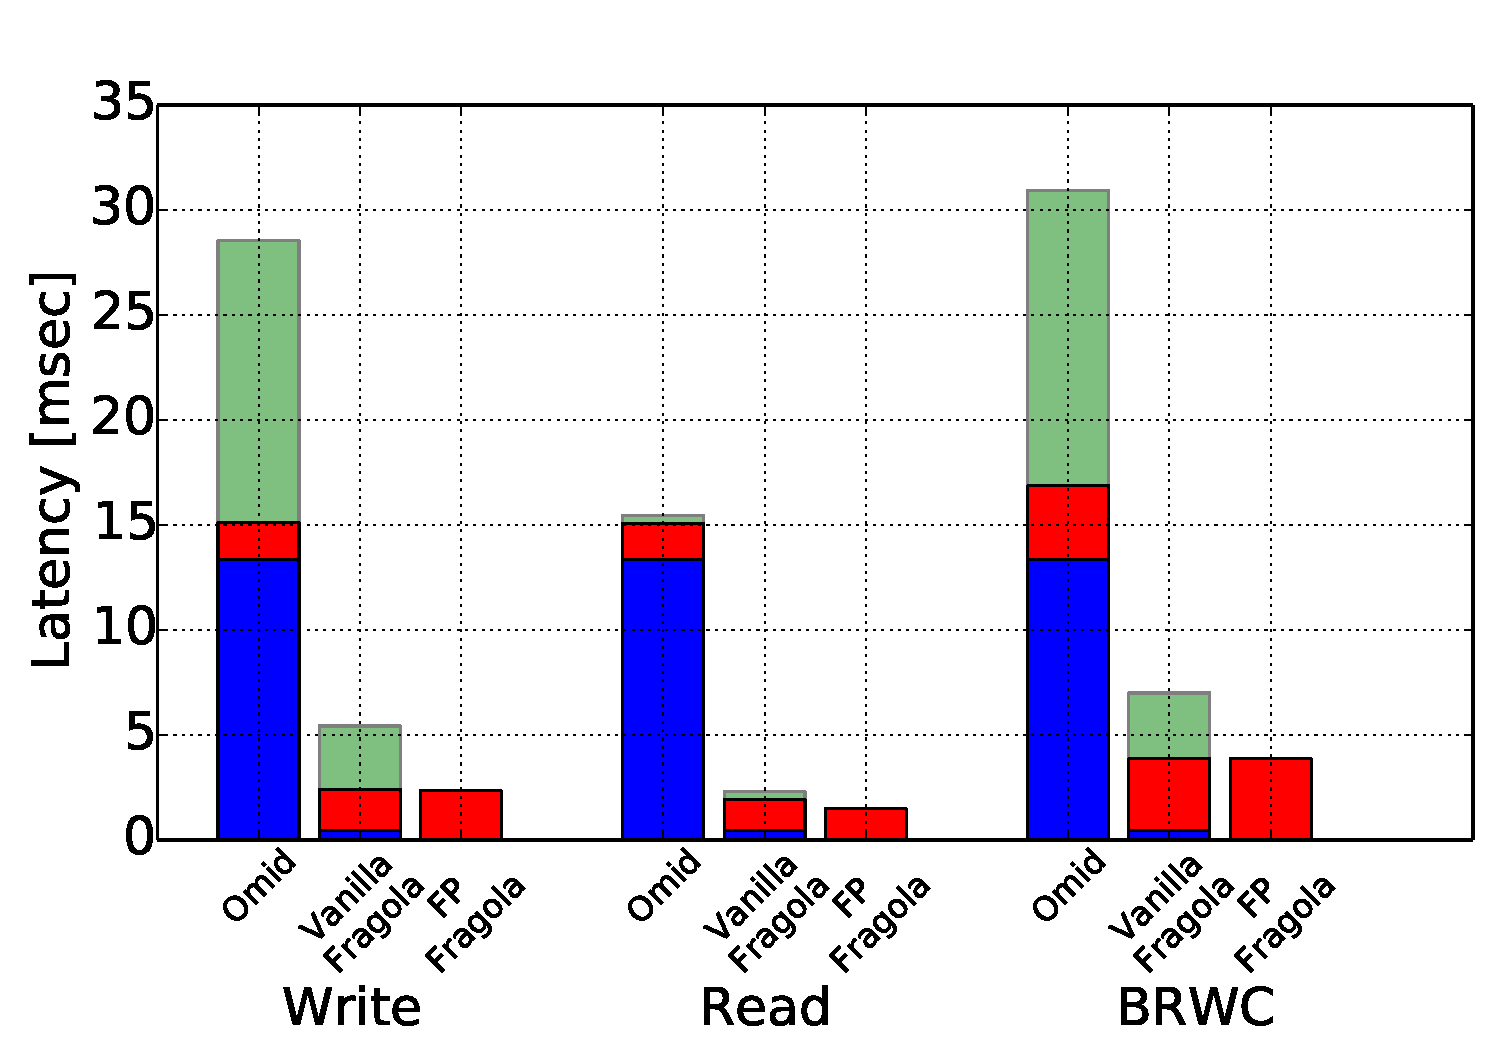
\includegraphics[width=\textwidth]{figs/latency_allPUTGET.pdf}
        \caption[]{Low load (100K tps).}
        \label{fig:stack-brc}

      \end{subfigure} 
    
& 
      \begin{subfigure}[t]{0.48\textwidth}
      	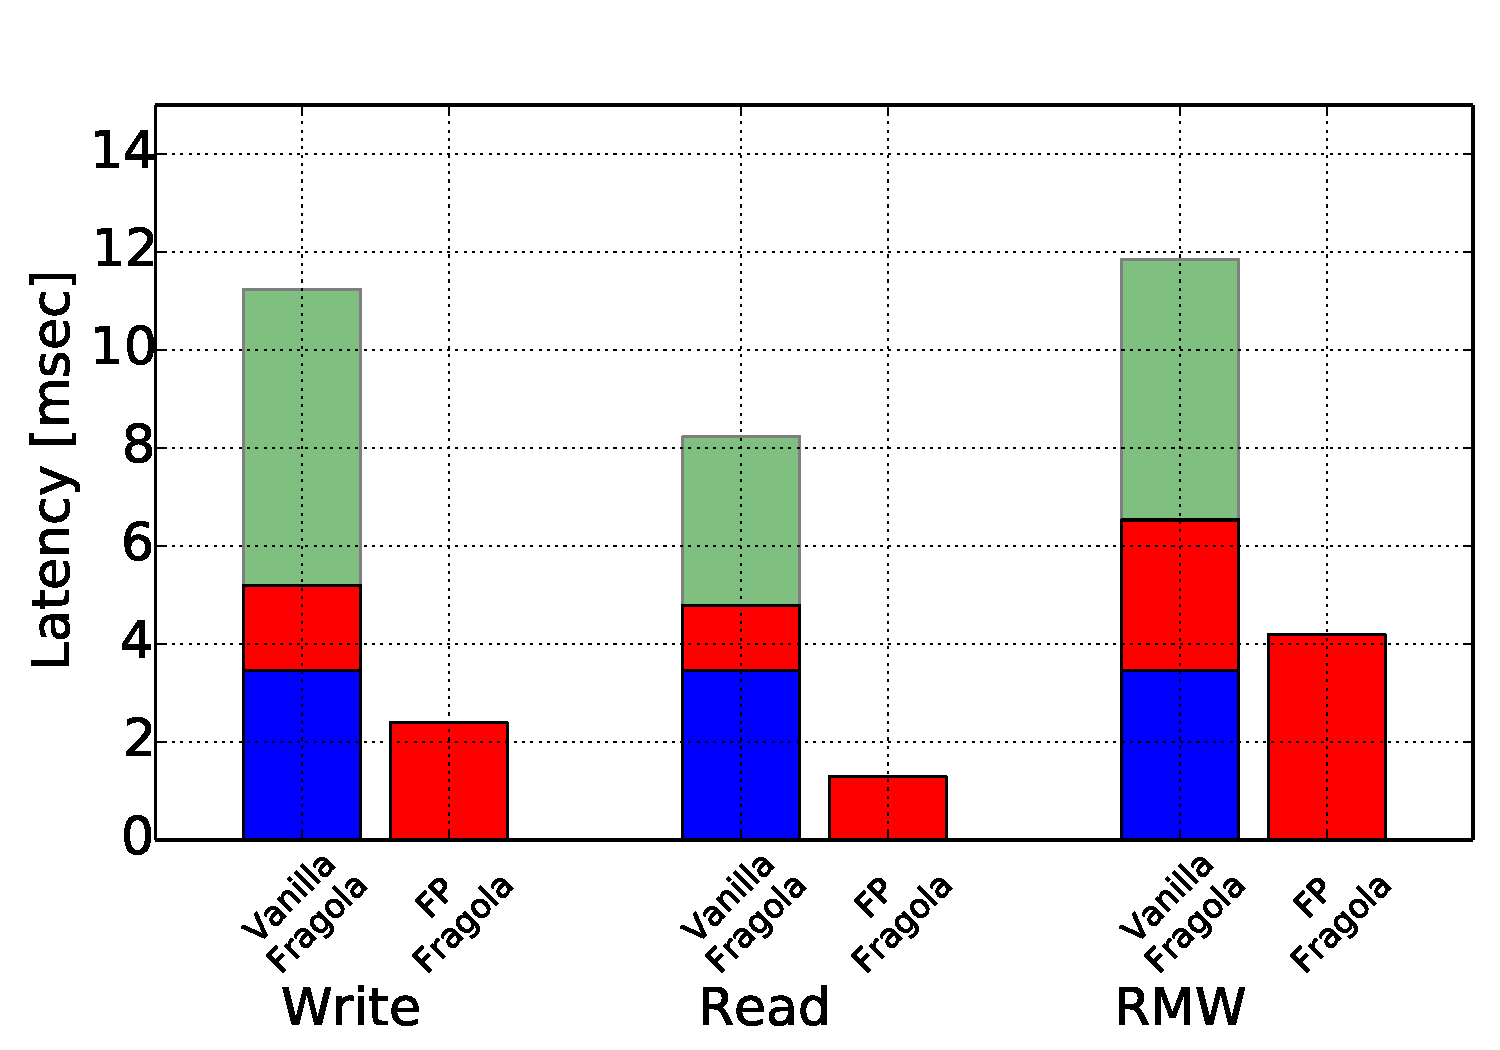
\includegraphics[width=\textwidth]{figs/latencyHighThrough_PUTGETRMW.pdf}
	\caption{High load (500K tps).}
	\label{fig:hightx}
      \end{subfigure}  & 

\end{tabular}
       \caption{Latency breakdown  for single-key transactions under  random mix workload. }
\end{figure*}


\subsection{Results}
\label{ssec:results}

\paragraph{Throughput and latency of short transactions.} 

Recall that \sys\ is motivated by the prevalence of short transactions in production, and is designed with
the goal of speeding such transactions up.
Its advantage is less pronounced for long transactions, where the cost of begin and commit is amortized
across many reads and writes.
To make the comparison meaningful, we classify transactions by their lengths and whether they
access a single key, and study each transaction class separately. 

We begin with short transactions. 
Figure~\ref{fig:tl-1} presents the average latency of single-key transactions run as part of the random mix,
as a function of {system} throughput.
Figure~\ref{fig:stack-brc}  then zooms in on the latency of such transactions under 
a throughput of 100K tps, and breaks up the different factors contributing to it. 
Figure~\ref{fig:hightx}  presents a similar breakdown under a high load of 500K tps; Omid 
is not included in the latter since it does not sustain such high throughput.

As we can see, under light load, \sys\ improves the latency of Omid by 4x to 5x, even without the fast path.
This is because in Omid, both begin and commit wait for preceding transactions to complete the writes of 
their commit entries; this stems from Omid's design choice to avoid the need for resolving pending write intents
by aborting transactions; see last (rightmost) column in Table~\ref{table:design-space}. 
Single-key writes suffer from both the begin and commit latencies, whereas single-key reads  
suffer only from begins (Figure~\ref{fig:stack-brc}). 

As load increases, Omid suffers from a well-pronounced bottleneck, and its latency at 200K tps is doubled, where \sys's 
latency is unaffected. The extra delay in Omid is due to batching of commit record updates, 
which its TM applies to handle congestion~\cite{Omid2017}. 
\sys, in turn, begins to experience a bottleneck (due to a heavy request load on the TM)  at 250K tps.
Such congestion arises due to Omid's centralized 
commit entry management (penultimate column in Table~\ref{table:design-space}).

The FP API delivers better performance for this traffic. For instance, under low load (Figure~\ref{fig:stack-brc}),
single writes take an average of 2.4ms using 
the {\code bwc} API versus 5.4ms using the regular transaction API (consisting of begin, write, and commit). 
For comparison, a native HBase write takes roughly 2ms under this load.
A single read executed using {\code brc} takes 1.5ms, which is the average latency of a native HBase read,
versus 2.3ms as a regular transaction. 
For transactions that read and write a single key as part of the BRWC workload, 
%Their latency breakdown under a 100K tps throughput is shown in Figure~\ref{fig:rmw}.
the fast path implementation (consisting of \code{br} and \code{wc} calls) completes within 3.9ms,
versus 7ms for Vanilla \sys\ and 30.9ms for Omid. 

Under high load (Figure~\ref{fig:hightx}), the fast path is more beneficial: it reduces the latency of write, read, and brwc from
ms, ms, and ms to ms, ms, and ms respectively. 



\paragraph{Long transactions.} 
We now examine longer transactions run as part of the random mix workload.
Figure~\ref{fig:throughput-latency} shows the results for transactions of lengths $5$ and $10$.
We see that the latency gap of \sys\ over Omid remains similar, but is amortized 
by other operations. Omid's control requests (begin and commit) continue to 
dominate the delay, and comprise $61\%$ of the latency of 10-access transactions.
In contrast, \sys's transaction latency is dominated by data access. For example, in 10-operation transactions only 
$17\%$ of the time is spent on the control path, which leads to much faster completion. 



\begin{figure*}[t]
\centering{
\begin{tabular}{cc}

    \begin{subfigure}[t]{0.48\textwidth}
	\includegraphics[width=\textwidth]{figs/throughputlatency10.pdf}
	\caption[]{Throughput versus latency, transaction size = 10}
    \label{fig:tl-10}
  \end{subfigure} & 


  \begin{subfigure}[t]{0.48\textwidth}
	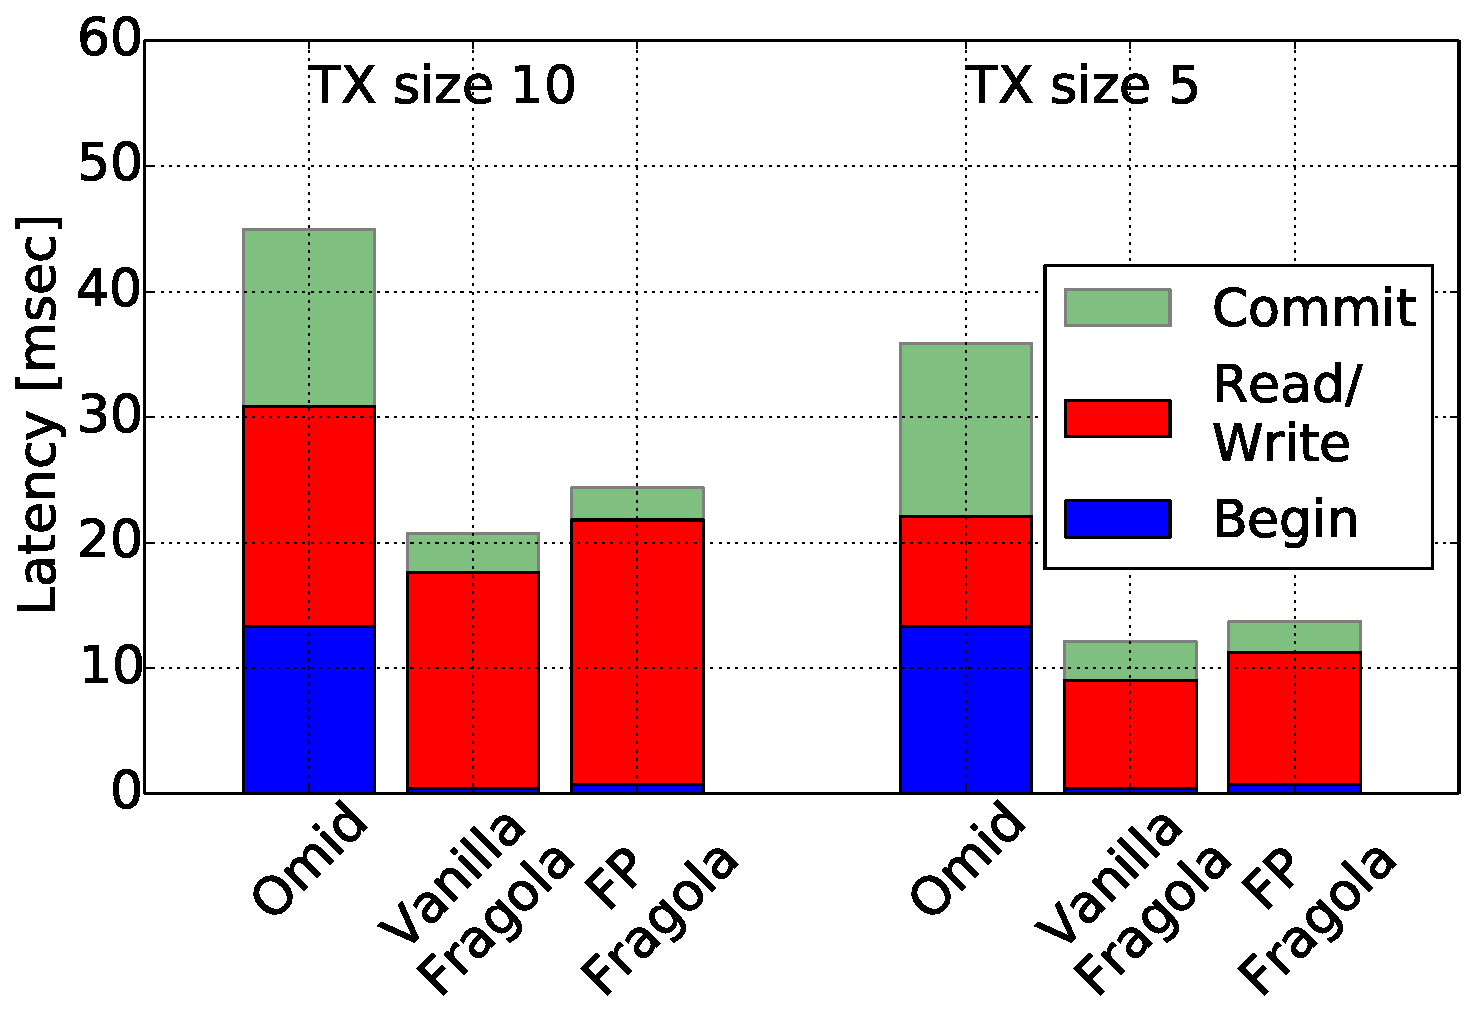
\includegraphics[width=\textwidth]{figs/latency_5_10.pdf}
	\caption[]{Latency breakdown, transaction size = 5, 10}
    \label{fig:stack-tx10}
  \end{subfigure} 
\end{tabular}  	
}		
  \caption{Latency vs.\ throughput  and latency breakdown  for long transactions in random mix workload. }
  \label{fig:throughput-latency}
\end{figure*}

Nevertheless,
the FP mechanism takes its toll on the data path, which resorts to atomic check\&mutate operations 
instead of simple writes. This is exacerbated for long transactions. 
For example, a 10-access transaction takes 24.4ms with FP \sys, 
versus 20.8ms with Vanilla \sys. 



\begin{figure}[h!]
\centering
\begin{subfigure}[t]{0.48\textwidth}
\centerline{
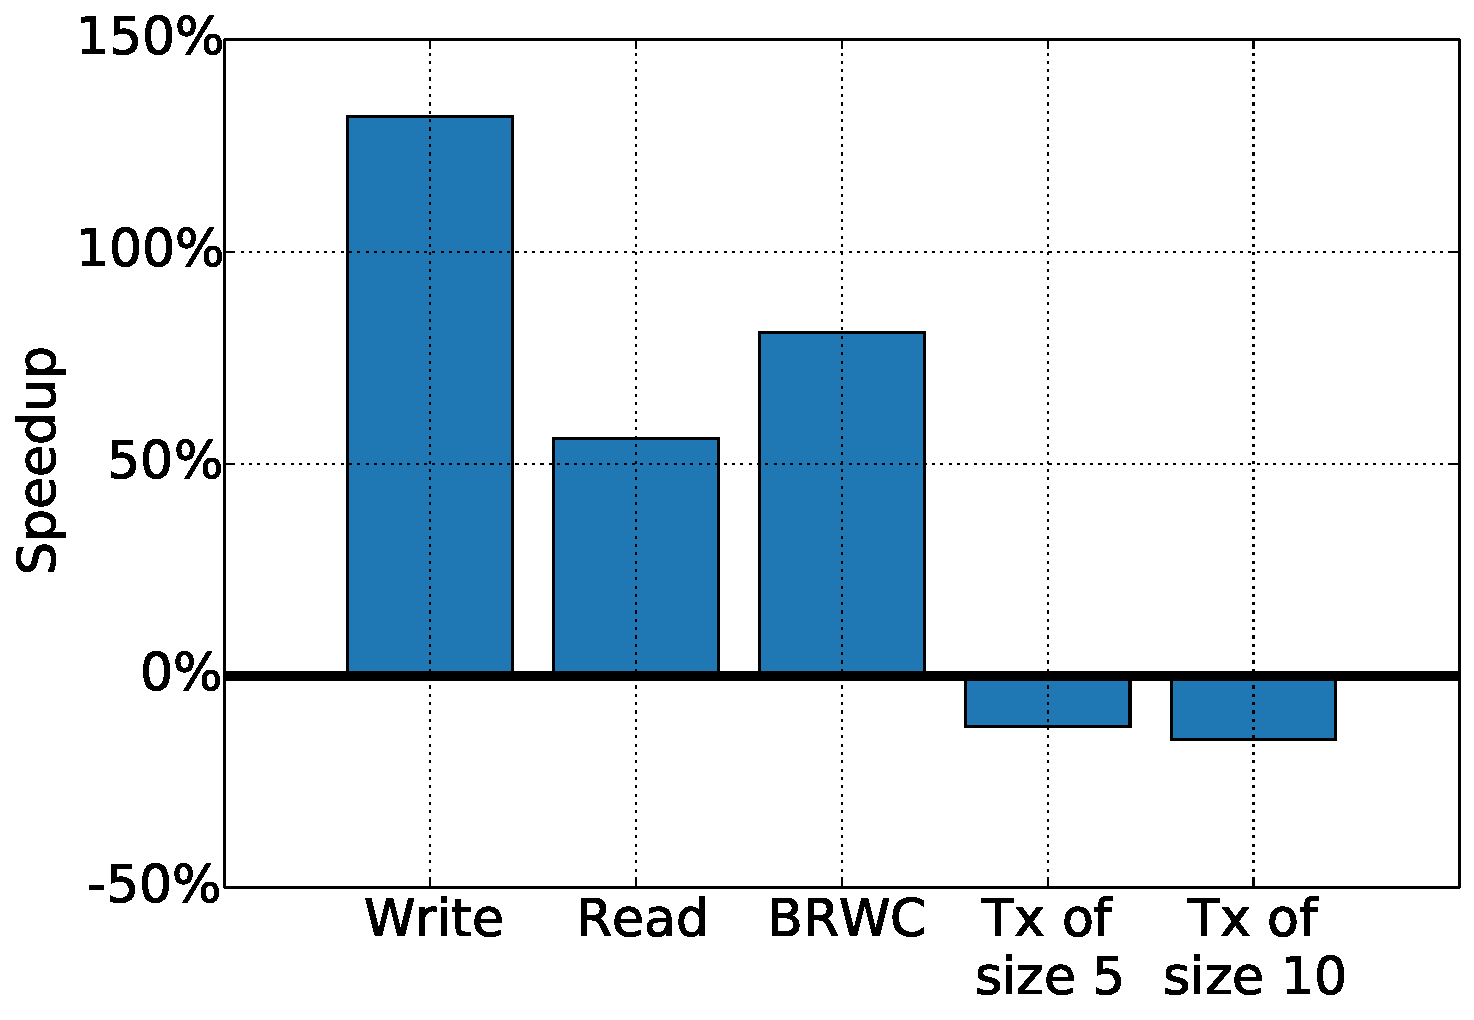
\includegraphics[width=.9\textwidth]{figs/low_speedup.pdf}
}
\caption{Low load (100 tps)} 
\end{subfigure} 
\begin{subfigure}[t]{0.48\textwidth}
\centerline{
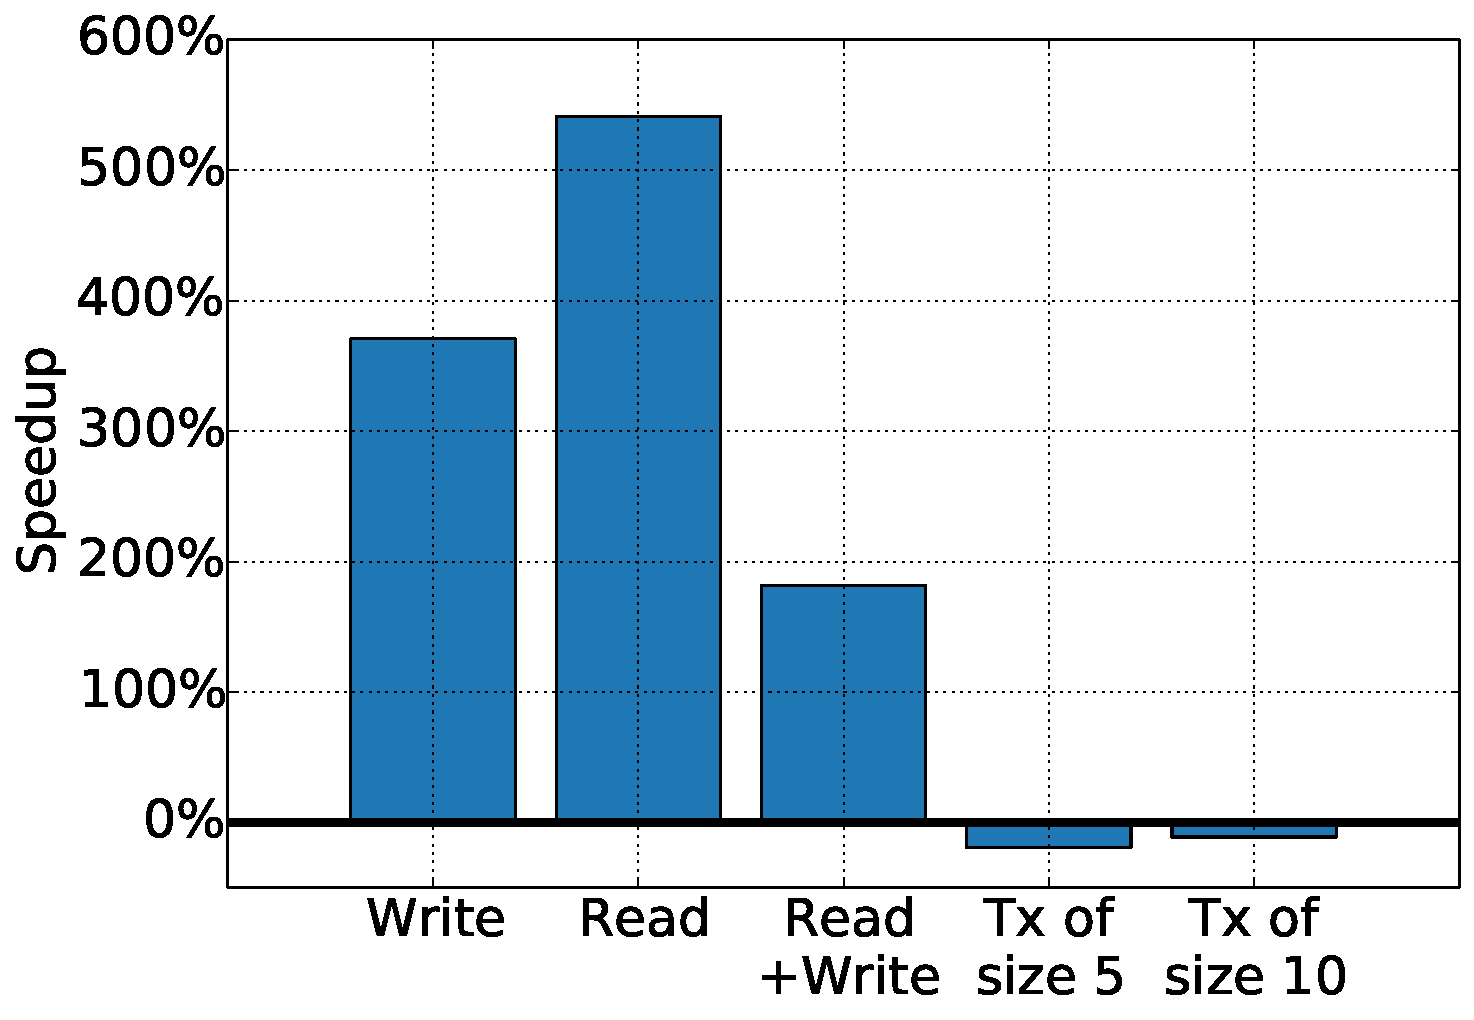
\includegraphics[width=.9\textwidth]{figs/high_speedup.pdf}
}
\caption{High load (500 tps)} 
\end{subfigure} 
\caption{Latency speedup with  fast path API in {\sys}.}
\label{fig:fp-tradeoff}
\end{figure}



Figure~\ref{fig:fp-tradeoff} summarizes the tradeoffs entailed by the fast path API
(relative to Vanilla \sys) for the different transaction classes. 
We see that the speedup for single-write transactions is 2.3x, whereas the worst slowdown is $14.8\%$. 
In systems geared towards real-time processing, this is a reasonable tradeoff, since long transactions 
are infrequent and less sensitive to extra delay. Under the studied workload, e.g.,   FP \sys\/ is more desirable. 



\paragraph{Abort rates.}

We note that \sys\/ yields slightly higher rates of transaction aborts compared to Omid 
(recall that Vanilla \sys\/ aborts tentative writes in favor of concurrent reads, whereas FP \sys\/ also aborts
singleton writes in presence of concurrent tentative writes). However, the abort rates exhibited by all  
the systems are minor. Here, under the highest contention, FP \sys\/ aborts approximately $0.1\%$ 
of the transactions vs Vanilla \sys's $0.08\%$ and Omid's $0.07\%$ 
(the latter  is in line with~\cite{Omid2017}).  
\remove{
}
